\subsection{Requirements}\label{sds_requirements}
Defining requirements for a design system that will serve as the foundation for an entire product area is no easy task. In the world of \ac{SaaS} products, there is no central place for best practices and guidelines. For this reason, this chapter looks at both functional and technical requirements. Functional requirements take the perspective of the various stakeholders in the system and model what requirements they might have for the system. For technical requirements, on the other hand, an exploration of ten design systems helps to identify the most important technical requirements for the \ac{SDS}.
\subsubsection{Functional requirements}
% Add use cases here
Functional requirements describe the necessary functionality of a software system. Hull et al. suggest modeling functional requirements using use case diagrams. These diagrams show the relationship between the acting roles and the presented system.\cite{hull_requirements_2011} \\
In the case of \ac{SDS}, there are two different types of interactions. There is an active interaction and a passive interaction. \\
Passive interaction means that any web application implements the design system, and the actor uses the design system passively by interacting with the web application. Since the web application uses components and policies of \ac{SDS}, the actor interacts with the design system under the hood. \\
On the other hand, active interaction is when an actor interacts directly with the design system. Directly means he accesses the design system documentation and its components and uses them to implement or design new applications. \\
Table \ref{tab:stakeholders_sds} provides a brief overview of the actors and their type of interaction with the \ac{SDS}.
\begin{table}[!ht]
    \begin{tabular}{|p{0.2\linewidth} | p{0.15\linewidth}| p{0.5\linewidth}|}
    \hline
     \textbf{Actor} &\textbf{Interaction} & \textbf{Description} \\ \hline
     Collaborator & Active & Collaborators are designers and developers who want to contribute to the design system. Often, these contributors are collaborators in other open source projects. However, companies do not pay for their work on the design system.   \\ \hline
     Users & Active & Users are developers and designers who use the design system to develop new products. They are the customers of the design system. They need support when creating their products. The design system makes their work easier.   \\ \hline
     End users & Passive & End users are all people who use \ac{SaaS} products in their daily work. They do not actively interact with the design system but with a web application that implements the design system. Therefore, they do not need to know whether the web application they use implements the design system.  \\ \hline
     
    \end{tabular}
    \caption{\label{tab:stakeholders_sds} Stakeholders of \ac{SDS}}
\end{table}
The personas presented are extraction of personas most likely to interact with the design system. The selected personas help create use cases describing the \ac{SDS}'s functional requirements. By looking at the system from the position of each actor, it is possible to formulate requirements for a design system that will serve as the basis for a \ac{SaaS} product. The type of interaction with the design system separates the following use case diagrams, starting with the passive interaction of the personas. \\

\begin{figure}[htbp]
    \centerline{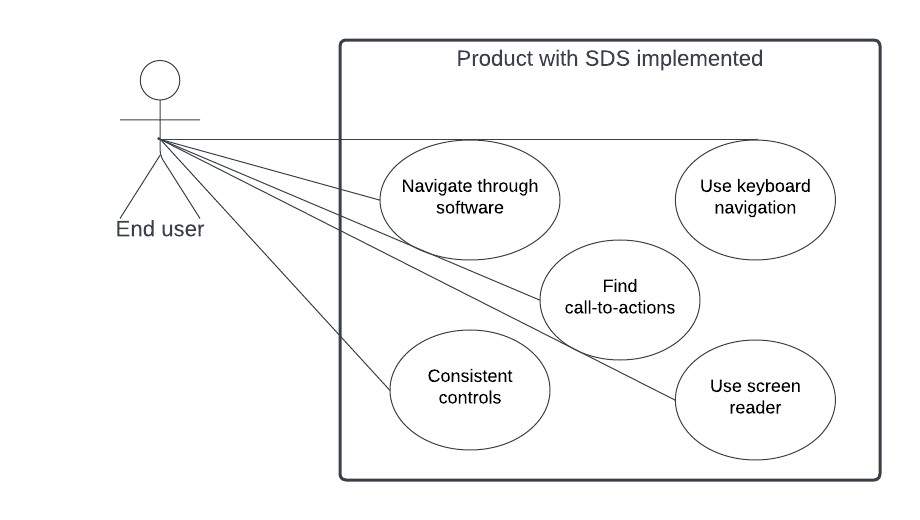
\includegraphics[width=\linewidth]{images/use_case_diagram_passive.png}}
    \caption{Use case diagram passive interaction with \ac{SDS}}
    \label{use_case_passive}
\end{figure}
Figure \ref{use_case_passive} shows the passive interaction with the SDS via a web application that implements the design system. The only actor, in this case, is the end users, as described in Table \ref{tab:stakeholders_sds}. \\ 
Actors passively interact with the design system through the web application, which leads to five use cases. Of course, there could be more use cases for the end users, but these are the five most important to consider for now. \\
\begin{enumerate}
    \item The design system should allow the end user to navigate the applications similarly. This requirement means that every application that implements the patterns and components of SDS has the same navigation structure. Therefore, end users do not have to get used to a new navigation structure when they switch to another application. 
    \item Controls in web applications should have the same arrangement for different applications. The end user does not have to learn how to submit a form or find the settings for their user profile. 
    \item Call-to-actions should have the same look and feel from application to application. This way, buttons on pages can be found quickly. This requirement will help the end user increase productivity. 
    \item End users may be temporarily or permanently unable to use the mouse. Therefore, it is essential for these users they can navigate through an application using the keyboard. The design system should be aware of this requirement. 
    \item End users may not be able to see the website temporarily or permanently. Therefore, these users must use a screen reader when interacting with the application. The design system should implement components so that a screen reader can read them.
\end{enumerate}
This enumeration completes the initial use cases for passive use of the SDS. \\

Compared to passive interaction with the design system, there are two types of actors in active interaction. Table \ref{tab:stakeholders_sds} shows both the collaborators and the users of the active interaction. Both actors create a variety of use cases. Some are used by only one actor, while others are shared. Figure \ref{use_case_active} shows a use case diagram for active interaction with the design system. \\
\begin{figure}[htbp]
    \centerline{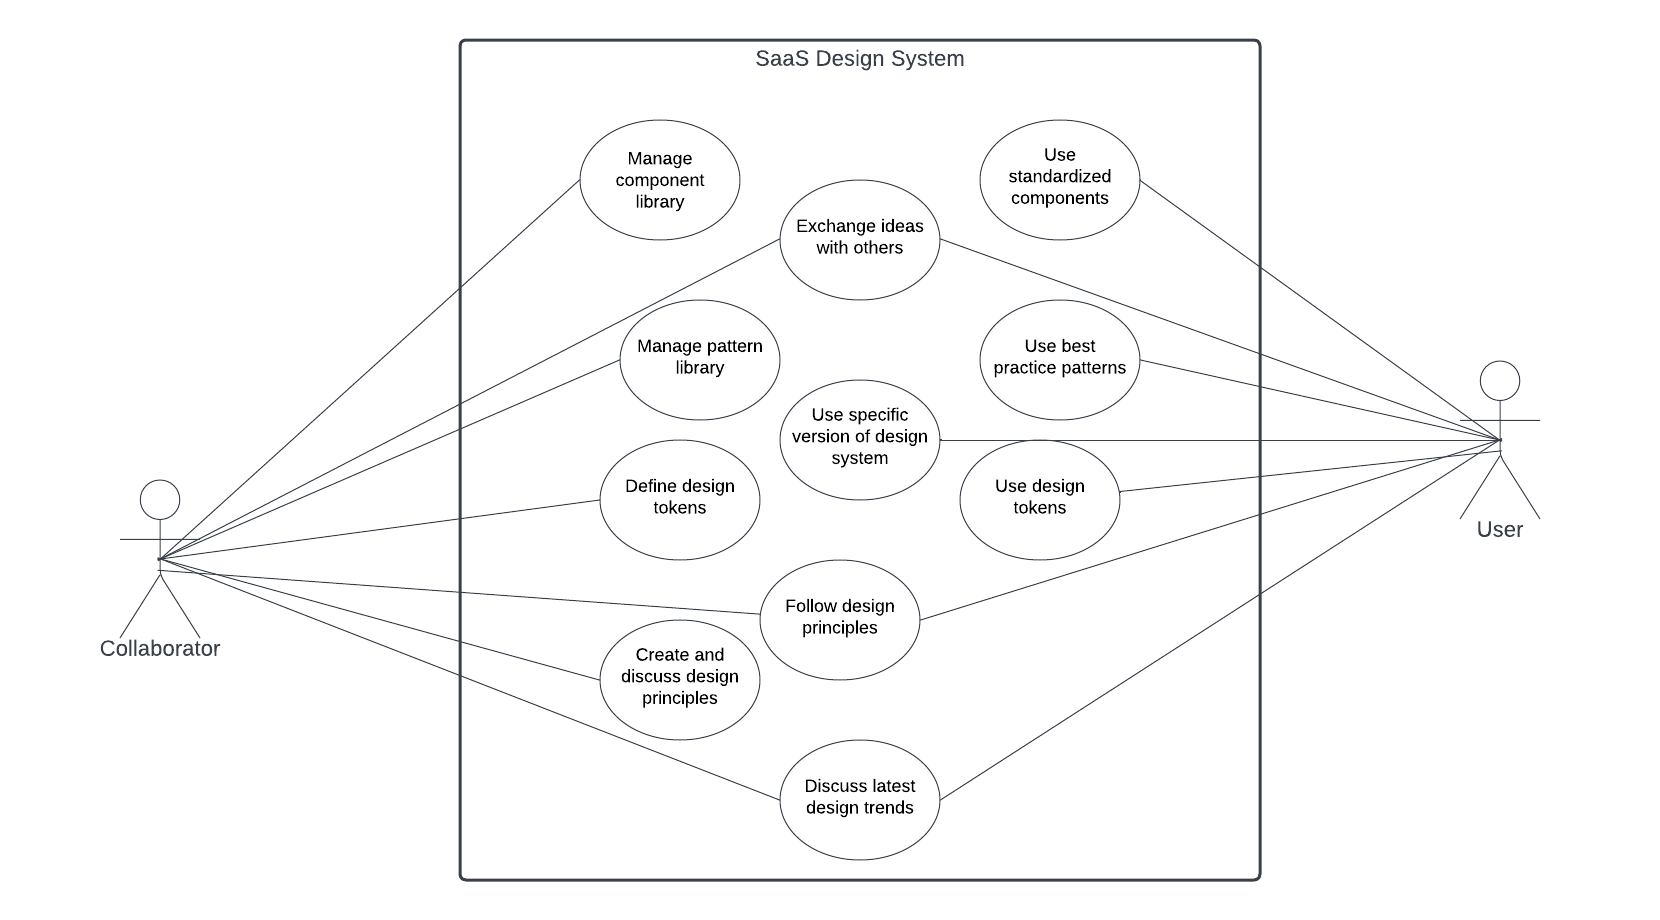
\includegraphics[width=\linewidth]{images/use_case_diagram_active.png}}
    \caption{Use case diagram active interaction with \ac{SDS}}
    \label{use_case_active}
\end{figure}
The visual representation of the use cases allows to separate them for further explanation.Therefore, the use cases just presented are divided into three categories, following the collaborator, the user, or both actors acting on a use case.\\

The first use cases for the \ac{SDS} to discuss are the collaborator ones:
\begin{enumerate}
    \item Collaborators want to manage, contribute and program new components of the design system's component library. It should be easy to contribute to such a design system.
    \item Collaborators want to manage and contribute to the patterns of a design system. Patterns need a process to define new patterns and discuss existing ones to improve them.
    \item Collaborators can create new design tokens. Design tokens define the basis for all components and patterns in the design system. 
    \item Collaborators want to discuss and adjust the design principles for the \ac{SDS} design system. The principles should not change too much, so an appropriate process should be defined to have a good management process.  
\end{enumerate}

The second category of use cases is use cases that relate only to the design system users. As described earlier, users only want to use the design system's provided assets and do not want to edit or create content on the design system itself.
\begin{enumerate}
    \item Users want to use the standardized components provided by the design system. The actions required to implement the component in the user's application should be as simple as possible.
    \item Users want to use the best practice patterns provided by the design system. The documentation and the guide according to the pattern should lead the users to an easy implementation.
    \item Users want to use the design tokens provided by the design system. Design tokens not only help style the components and patterns provided by the design system but also support components and structures created by the user's application. This support results in a consistent style throughout the application, whether or not users use the design system components. 
    \item Users do not want to destroy their running applications that implement the design system. Therefore, it is essential to provide for the versioning of the design system. They also need to be able to use older versions of the design system when needed and decide when to upgrade the application to the latest version. 
\end{enumerate}
Last but not least, the use cases of both actors need further details. These use cases are notable because they address both parties. A detailed look at these cases shows what they are.
\begin{enumerate}
    \item Active stakeholders should have the opportunity to exchange ideas and thoughts on a platform such as a shared design system. New content for the design system can emerge from these interactions. A community can form around it with a communication platform for the design system.  
    \item Both stakeholder groups want to follow the design principles when creating new components, whether for their applications or the design system. This point doubles the importance of design principles within a design system. The goal of a design system is to make them simple, accessible, and understandable. 
    \item Active actors on the SDS want to be informed about the latest trends and best practices in \ac{SaaS} applications. Therefore, a design system should provide an option to publish news on these topics. Such a platform will lead to more interaction on the design system and motivate stakeholders to discuss improvements.
\end{enumerate}

These enumerations and diagrams summarize the functional requirements for the \ac{SDS}. Of course, the number of use cases for such a design system is much larger, but this elaboration focuses on the most important ones. When the system is in use, there could be many more use cases in the future. However, this should be an iterative process driven by the community that forms around the system. 

\subsubsection{Technical requirements}
In addition to functional requirements, there are also technical requirements. Technical requirements describe the technical details of a design system. This elaboration defines the technical requirements looking into \ac{SaaS} product design systems and design systems that share a common purpose. With this data, it is possible to extract technical requirements when implementing such a design system.\\
The research aims to identify best practices from the \ac{SaaS} world and understand the needs of companies that use design systems. In addition, when looking at broader design systems with a common purpose, there is an excellent opportunity of finding a reference design system. Table \ref{tab:design_systems_in_the_wild} lists the studies of ten design systems with a summary.
% \newpage
% \begin{table}[!ht]
\begin{longtable}{|p{0.2\linewidth} | p{0.7\linewidth}|}
\hline
 \textbf{Name} & \textbf{Description} \\ \hline
ServiceNow \cite{servicenow_servicenow_nodate}  & Platform design system.  Guidance to create components and upload them to the platform. \\ \hline
Adobe Spectrum  \cite{spectrum_adobe_spectrum_nodate} & User centralised design system. Many well designed components with matching guide to deliver a great experience. Built in web components and react components. \\ \hline
Zendesk Garden \cite{zendesk_garden_zendesk_nodate} & Basic design system with guidelines, components and patterns. Tailwindcss integration. Built in react components. \\ \hline

Atlassian Design System \cite{atlassian_design_system_atlassian_nodate} & Design System connected with company values. A lot of guides on how to use designs, components and to write content. Includes also employee motivation. Built in react components. \\ \hline
Base Web  \cite{base_base_nodate} & Open source design system. Used by Uber. Providing a blog and guides on how to use the base design system. Design System intended to be used as baseline and should be overwritten when used. No principles or values included. \\ \hline
SAP Fiori  \cite{sap_fiori_nodate} & Standard design system. Focus on accessibility and multiple device support. Including many themes for different applications. Delivers a toolkit to better use the design system as a designer.  \\ \hline
GOV UK Design System  \cite{govuk_govuk_nodate} & Not really a design system. Missing guidelines and principles. Externals can propose changes. Providing \ac{CSS} classes for \ac{HTML} elements.  \\ \hline
Lightning Design System \cite{lightning_design_system_lightning_nodate} & Design System to support developers and designer at their work. 4 principles with a clear message to align every user. Guidelines and best practices on many topics.  Components are built with pure \ac{CSS} classes. \\ \hline
Google Matrial Design \cite{google_material_2022} & Open source design system. Providing the user with design principles which helps to understand the usage of the design system. Material Design provides only components and no patterns. Blogs and further resources are helping additionally to the guidelines. Components are built with pure \ac{CSS} classes. \\ \hline
Pluralslight Design System \cite{pluralsight_ds_nodate} & Design System without principles and guidelines. For the moment only components are present. Providing a workflow for developers and designers to contribute to the design system.  Only few patterns. Built with react components.  \\ \hline
\caption{\label{tab:design_systems_in_the_wild} Overview of 10 existing design systems}
\end{longtable}
% \end{table}
The analysis of the design systems listed above derives three central technical requirements. These requirements serve as a guide for the development of the design system.
\begin{enumerate}
    \item A good reference for a design system with a suitable use case is the Base Web Design System. Its purpose of providing a base of styles and functional components helps developers to extend the design system and create their own for their products. Also, the fact that this design system is open source underlines that the community is developing this design system, not a corporate design team. As a shared design system, it focuses mainly on accessibility and internationalization. The tutorial explains extending and using the design system, a perfect reference model for \ac{SDS}.  
    \item A look at Google's Material Design shows that even an open source and versatile design system can have design principles. Design principles help developers understand how to develop and design the system. Therefore, design principles are essential for a standard design system like \ac{SDS}. 
    \item Another reasonable assumption for \ac{SDS} is adaptability. Examination of some design systems shows that some use a frontend framework to develop their components. This building block ties the users of the design system to a framework. However, design systems such as GOV UK and Salesforce's Lightning Design System do not use frameworks. Their components consist solely of web standards such as \ac{HTML} and \ac{CSS}. Therefore, the exclusive use of web standards is a requirement for the \ac{SDS}. 
\end{enumerate}

In all the design systems listed in Table \ref{tab:design_systems_in_the_wild}, many more requirements could be helpful for a design system that serves as a basis for others. Due to the limitation of this elaboration, this chapter only presented the three main aspects. \\




